\documentclass[border=10pt]{standalone}
% Shared style for the EMONI diagrams. Build: tectonic <file>.tex, then pdftocairo -svg.
\usepackage{fontspec}
\setmainfont{FiraSans}[Extension=.otf,UprightFont=*-Regular,BoldFont=*-SemiBold,ItalicFont=*-Italic,BoldItalicFont=*-SemiBoldItalic]
\setmonofont{FiraMono}[Extension=.otf,UprightFont=*-Regular,BoldFont=*-Medium,Scale=0.9]
\usepackage{tikz}
\usetikzlibrary{arrows.meta,positioning,shapes.geometric,shapes.misc,calc,fit,backgrounds}
\definecolor{eg}{HTML}{11903B}   % EMONI green
\definecolor{egl}{HTML}{E8F7EE}
\definecolor{eb}{HTML}{2A78D6}   % blue
\definecolor{ebl}{HTML}{EAF2FC}
\definecolor{eo}{HTML}{D9631E}   % orange
\definecolor{eol}{HTML}{FDF0E7}
\definecolor{ep}{HTML}{7C4DCC}   % purple
\definecolor{epl}{HTML}{F2ECFB}
\definecolor{er}{HTML}{C5221F}   % red
\definecolor{erl}{HTML}{FCEAEA}
\definecolor{ink}{HTML}{1F2328}
\definecolor{mute}{HTML}{59636E}
\definecolor{line}{HTML}{D0D7DE}
\tikzset{
  every node/.style={text=ink,font=\small},
  >={Stealth[length=2.4mm]},
  % sequence diagrams
  life/.style={draw=line,dashed,thick},
  head/.style={draw=#1,fill=#1!8,rounded corners=3pt,minimum width=27mm,minimum height=11mm,align=center,font=\small\bfseries,thick},
  act/.style={draw=#1,fill=#1!18,minimum width=2.2mm},
  msg/.style={->,thick,draw=ink},
  ret/.style={->,dashed,draw=mute},
  mlabel/.style={font=\footnotesize,fill=white,inner sep=1.5pt,align=center},
  note/.style={draw=#1,fill=#1!8,rounded corners=2pt,font=\footnotesize,align=left,inner sep=4pt},
  frag/.style={draw=mute,rounded corners=2pt},
  fraglabel/.style={draw=mute,fill=white,font=\footnotesize\bfseries,inner sep=2.5pt,anchor=north west},
  % activity diagrams
  start/.style={circle,fill=ink,minimum size=4mm,inner sep=0},
  stop/.style={circle,draw=ink,thick,minimum size=5mm,inner sep=0,path picture={\fill[ink] (path picture bounding box.center) circle (1.4mm);}},
  step/.style={draw=#1,fill=#1!8,rounded corners=5pt,thick,minimum height=9mm,minimum width=40mm,align=center,font=\small},
  step/.default=eg,
  dec/.style={diamond,aspect=2.2,draw=ink,fill=white,thick,inner sep=1.5pt,align=center,font=\footnotesize},
  flow/.style={->,thick,draw=ink},
  guard/.style={font=\footnotesize\itshape,text=mute,fill=white,inner sep=1.5pt},
  lane/.style={draw=line,fill=#1,rounded corners=4pt},
  lanetitle/.style={font=\small\bfseries,text=mute},
}

% Sequence: flashing and measuring a bench device from anywhere.
\begin{document}
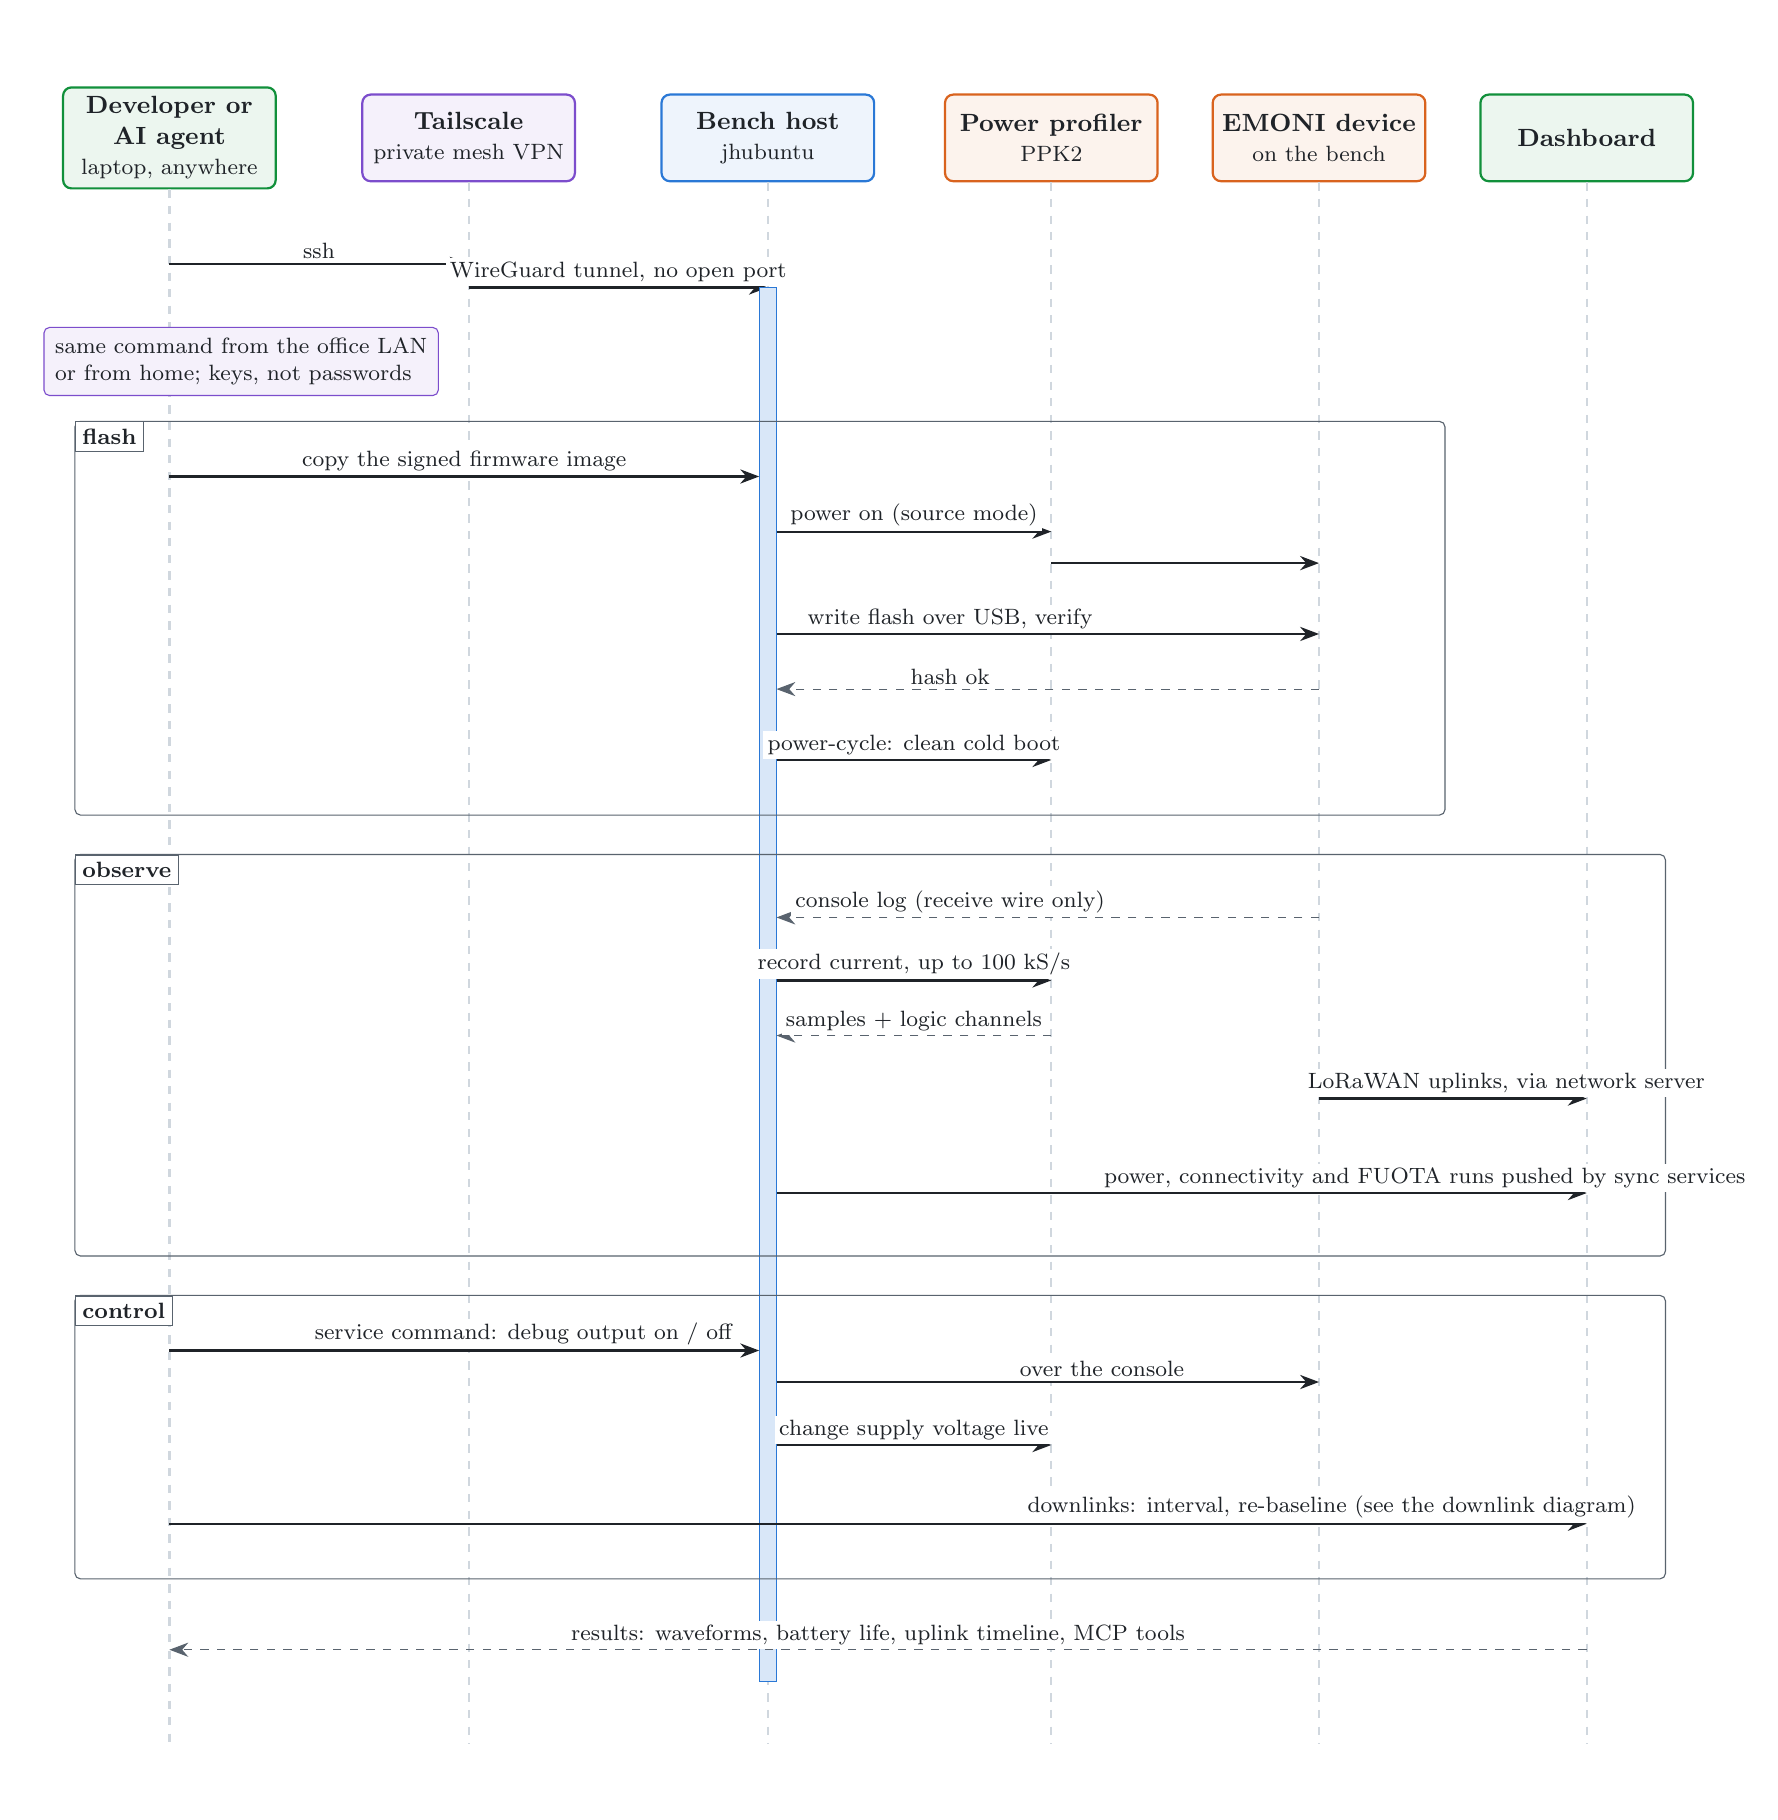
\begin{tikzpicture}[x=1cm,y=1cm]
\fill[white] (-1.8,1.4) rectangle (19.4,-21.0);
\def\B{-20.4}
\foreach \x/\n/\c/\t in {0/dev/eg/Developer or\\AI agent\\{\footnotesize\mdseries laptop, anywhere},
                         3.8/ts/ep/Tailscale\\{\footnotesize\mdseries private mesh VPN},
                         7.6/hil/eb/Bench host\\{\footnotesize\mdseries jhubuntu},
                         11.2/ppk/eo/Power profiler\\{\footnotesize\mdseries PPK2},
                         14.6/brd/eo/EMONI device\\{\footnotesize\mdseries on the bench},
                         18.0/dash/eg/Dashboard}{
  \node[head=\c] (\n) at (\x,0) {\t};
  \draw[life] (\n.south) -- (\x,\B);
}
\draw[msg] (0,-1.6) -- node[mlabel,above]{ssh} (3.8,-1.6);
\draw[msg] (3.8,-1.9) -- node[mlabel,above]{WireGuard tunnel, no open port} (7.6,-1.9);
\node[note=ep,anchor=north west] at (-1.6,-2.4) {same command from the office LAN\\or from home; keys, not passwords};
\draw[act=eb] (7.49,-1.9) rectangle (7.71,-19.6);
% flash
\draw[frag] (-1.2,-3.6) rectangle (16.2,-8.6);
\node[fraglabel] at (-1.2,-3.6) {flash};
\draw[msg] (0,-4.3) -- node[mlabel,above]{copy the signed firmware image} (7.49,-4.3);
\draw[msg] (7.71,-5.0) -- node[mlabel,above]{power on (source mode)} (11.2,-5.0);
\draw[msg] (11.2,-5.4) -- (14.6,-5.4);
\draw[msg] (7.71,-6.3) -- node[mlabel,above,pos=0.32]{write flash over USB, verify} (14.6,-6.3);
\draw[ret] (14.6,-7.0) -- node[mlabel,above,pos=0.68]{hash ok} (7.71,-7.0);
\draw[msg] (7.71,-7.9) -- node[mlabel,above]{power-cycle: clean cold boot} (11.2,-7.9);
% observe
\draw[frag] (-1.2,-9.1) rectangle (19.0,-14.2);
\node[fraglabel] at (-1.2,-9.1) {observe};
\draw[ret] (14.6,-9.9) -- node[mlabel,above,pos=0.68]{console log (receive wire only)} (7.71,-9.9);
\draw[msg] (7.71,-10.7) -- node[mlabel,above]{record current, up to 100 kS/s} (11.2,-10.7);
\draw[ret] (11.2,-11.4) -- node[mlabel,above]{samples + logic channels} (7.71,-11.4);
\draw[msg] (14.6,-12.2) -- node[mlabel,above,pos=0.7]{LoRaWAN uplinks, via network server} (18,-12.2);
\draw[msg] (7.71,-13.4) -- node[mlabel,above,pos=0.8]{power, connectivity and FUOTA runs pushed by sync services} (18,-13.4);
% control
\draw[frag] (-1.2,-14.7) rectangle (19.0,-18.3);
\node[fraglabel] at (-1.2,-14.7) {control};
\draw[msg] (0,-15.4) -- node[mlabel,above,pos=0.6]{service command: debug output on / off} (7.49,-15.4);
\draw[msg] (7.71,-15.8) -- node[mlabel,above,pos=0.6]{over the console} (14.6,-15.8);
\draw[msg] (7.71,-16.6) -- node[mlabel,above]{change supply voltage live} (11.2,-16.6);
\draw[msg] (0,-17.6) -- node[mlabel,above,pos=0.82]{downlinks: interval, re-baseline (see the downlink diagram)} (18,-17.6);
\draw[ret] (18,-19.2) -- node[mlabel,above,pos=0.5]{results: waveforms, battery life, uplink timeline, MCP tools} (0,-19.2);
\end{tikzpicture}
\end{document}
